\chapter{The sky: what the reference cannot explain}\label{ch:sky}

\section{The idea}

After component separation, a CMB map is what the foreground model cannot explain. The methylome's counterpart is the \emph{sky}: at each
site, how far the specimen sits from what its healthy reference predicts, in units of the healthy spread. A healthy specimen reads a quiet sky,
$z$ centred on zero with no structure. A cell far from its healthy state, or a cell the reference does not hold, leaves structure.

\section{The sky chain v3 draws}

Chain v3 draws the sky on the neutrophil's 6,000 identity sites, in genome order (Stage~MC, \texttt{conductor\_v3.py}):
\begin{equation}
  z_i=\frac{H(\beta_i)-H(\mathrm{ref}_i)}{s_i},
  \label{eq:sky}
\end{equation}
with $H(\mathrm{ref}_i)$ the healthy neutrophil mean entropy at site $i$ for isolated cells, or $H(e_i)$ from the specimen's own composition for whole
blood (Eq.~\ref{eq:metawb}), and $s_i$ the spread of $H$ at that site across the six physical reference arrays, shrunk toward the pooled spread
(\texttt{neutrophil\_reference\_v1\_1.json}). \derived{} (the construction); $s_i$ is \calibrated. The noise term comes from purified reference cells,
not from a panel of people. Two numbers are taken from the map: the Met-A C-score (Chapter~\ref{ch:cscore}) and the fraction of sites with $|z|>3$, both
printed with every reading. What the map looks like on healthy and damaged arrays is in Chapter~\ref{ch:skytools}.

In whole blood the residual also carries composition error, so the whole-blood map is wider than the isolated-cell map: on the acceptance run the C-score
read 0.69--1.21 on isolated neutrophils and 0.78--1.49 on whole bloods (\texttt{chain\_tests/\allowbreak{}CHAIN\_V3\_ACCEPTANCE\_RUN3.md}). \measured{} No band is
set for either.

\section{The whole-array sky}

A sky over every address on the array, not only the identity sites, would show what the eight blood groups of Stage~A cannot explain anywhere in the
genome. Chain v3 does not draw it. Three things are needed first: a noise term for every address that comes from the array and the reference, not from
other people; a sex mask or a reference of the same sex, because the X chromosome lights up when a female array is read against male references
(Chapter~\ref{ch:skytools}); and a reference holding more than eight groups. \openprob

\section{The cell-count floor}

At multipole $\ell$ the CMB offers $2\ell+1$ independent modes, and the fractional uncertainty on the power there can never fall below
$\sqrt{2/(2\ell+1)}$ however good the telescope. A specimen has the same kind of limit. At a site with true methylation $\beta$ in a specimen of $N$
genome copies, the measured fraction has binomial standard deviation
\begin{equation}
  \sigma_{\mathrm{copies}}=\sqrt{\frac{\beta(1-\beta)}{2N}}
  \label{eq:cellcount}
\end{equation}
for diploid DNA. \derived{} Figure~\ref{fig:cellcount} sets it against array noise. For a whole-blood draw with millions of cells the copy-number floor is
negligible. For plasma cell-free DNA, which carries of order $10^4$ genome equivalents per millilitre-scale draw, it is $0.003$ at $\beta=0.7$, below array
noise at a single site but not negligible for a cell present at one per cent, whose contribution comes from about a hundred genomes. \calc{} The chain does
not yet carry this floor in any interval. \openprob

\begin{figure}[t]\centering
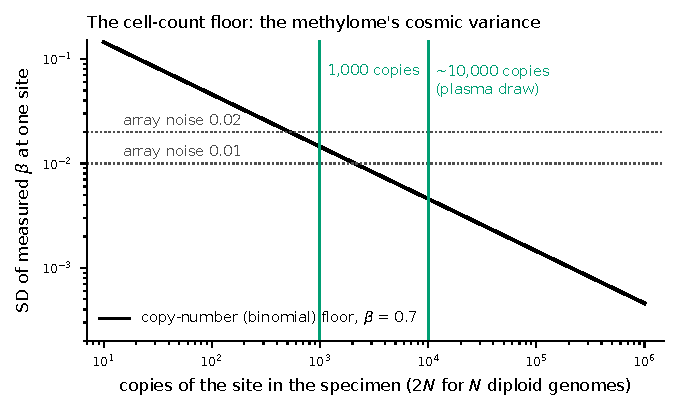
\includegraphics[width=0.8\textwidth]{figures/part4/fig_cell_count_floor.pdf}
\caption{Standard deviation of measured $\beta$ at one site from the finite number of genome copies (Eq.~\ref{eq:cellcount}, $\beta=0.7$, diploid), against
array measurement noise of 0.01 and 0.02. Vertical lines mark $10^3$ genomes and the $\sim10^4$ genome equivalents of a plasma draw. \calc}
\label{fig:cellcount}
\end{figure}

\section{A cleaner sky: the out-of-span map}

A residual after composition mixes two things: error in the solved fractions of known cells, and signal from cells the reference does not hold. They can be
separated exactly. Any mixture of the reference's cells, at any fractions, lies in the span of the cells' profiles. Projecting the residual onto that span and
onto its complement,
\begin{equation}
  \mathbf r=\underbrace{P_{\mathrm{span}}\mathbf r}_{\text{composition error}}+\underbrace{(I-P_{\mathrm{span}})\mathbf r}_{\text{what no known mixture can make}},
  \label{eq:outspan}
\end{equation}
leaves an out-of-span map that a composition error cannot move at all. \derived{} It is the direct counterpart of template cleaning on the sky. Its tests are
written before any specimen is projected (\texttt{doors/\allowbreak{}PROC\_OUTSPAN\_01\_PREREG.md}): a constructed specimen of known cells must read quiet; the map must
stay quiet when the known cells' fractions are thrown off by $\pm50$~\%; cells held out of the reference, spiked in at 1--10~\%, must be detected, in at least 12 of 16 cells at 5~\%; and between two
draws of one person a change of composition must read quiet while a newly added unknown cell appears. \prediction{} The pre-registration is written for the multi-source atlas of
Chapter~\ref{ch:atlas}. The map is not built in chain v3, whose reference spans eight blood groups, and the procedure has not run. \openprob
